\section{Theorie}
\label{sec:Theorie}
Trifft $\gamma$- oder $\beta$-Strahlung auf Materie, so finden Wechselweirkung
zwischen der Materie und der Strahlung statt, die die Strahlung abschwächen. Um
diese Wechselwirkung quantitativ beschreiben zu können, wird der Wirkungsquerschnitt
$\sigma$ definiert. Dieser ist ein Maß für die Häufigkeit der Wechselwirkung: Je größer
der Wirkungsquerschnitt $\sigma$, desto häufiger tritt die Wechselwirkung auf.
Zusätzlich hängt die Anzahl der Wechselwirkungen von der Dicke des Absorbermaterials ab.
Für $\gamma$-Strahlung ergibt sich für die Anzahl der Teilchen, die den Absorber
durchqueren können der exponentielle Zusammenhang
\begin{equation}
  N(D)=N_0 e^{-n \sigma D} \,.
  \label{eqn:absorptionsgesetz}
\end{equation}
Dabei beschreibt $N_0$ die Teilchenanzahl vor dem Absoprtionsvorgang, $n$ die
Teilchenanzahl in einer Volumeneinheit des Absorbermaterials, $\sigma$ den Wirkungsquerschnitt
und $D$ die Dicke des Absorbers. Die Teilchenanzahl im Absorber ist gegeben durch
\begin{equation}
 n=\frac{z N_{\symup{A}}}{V_{\symup{mol}}}=\frac{z N_{\symup{A}} \rho}{M} \,,
\end{equation}
wobei $z$ die Kernladungszahl des Absorbermaterials, $N_{\symup{A}}$ die Avogadrokonstante,
$V_{\symup{mol}}$ das Molvolumen des Absorbermaterials, $\rho$ die Dichte desselben und
$M$ das Molekulargewicht des Absorbermaterials ist.
Häufig  wird die Größe $n \sigma =\mu$ als der Absorptionskoeffizient bezeichnet.
Für sehr kleine Absorberdicken lässt sich das Absorptionsgesetz \eqref{eqn:absorptionsgesetz}
auch auf $\beta$-Strahlung anwenden.


\subsection{Theoretische Grundlagen der Gamma-Strahlung} %$\gamma$-Strahlung} || LATEX will irgenwie keine griechischen Buchstaben in Überschriften....
\label{subsec:gamma}

$\gamma$-Strahlung entsteht, indem Atomkerne von einem energetisch höheren in einen
energetisch niedrigeren Zustand fallen. Die überschüssige Energie wird in Form eines
$\gamma$-Quants mit der Energie
\begin{equation}
  E_{\symup{\gamma}}= E_1 - E_2
\end{equation}
abgegeben. Dabei bezeichnet $E_1$ den energetisch höheren und $E_2$ den energetisch
niedrigeren Zustand. Da die Zustände der Atomkerne diskret sind, weist auch das
Spektrum der $\gamma$-Strahlung scharfe Linien auf.

Bei der Wechselwirkung von $\gamma$-Strahlung mit Materie können verschiedene
Effekte auftreten. Diese sind in Abbildung \ref{fig:wechselwirkung} dargestellt.

\begin{figure}
  \centering
  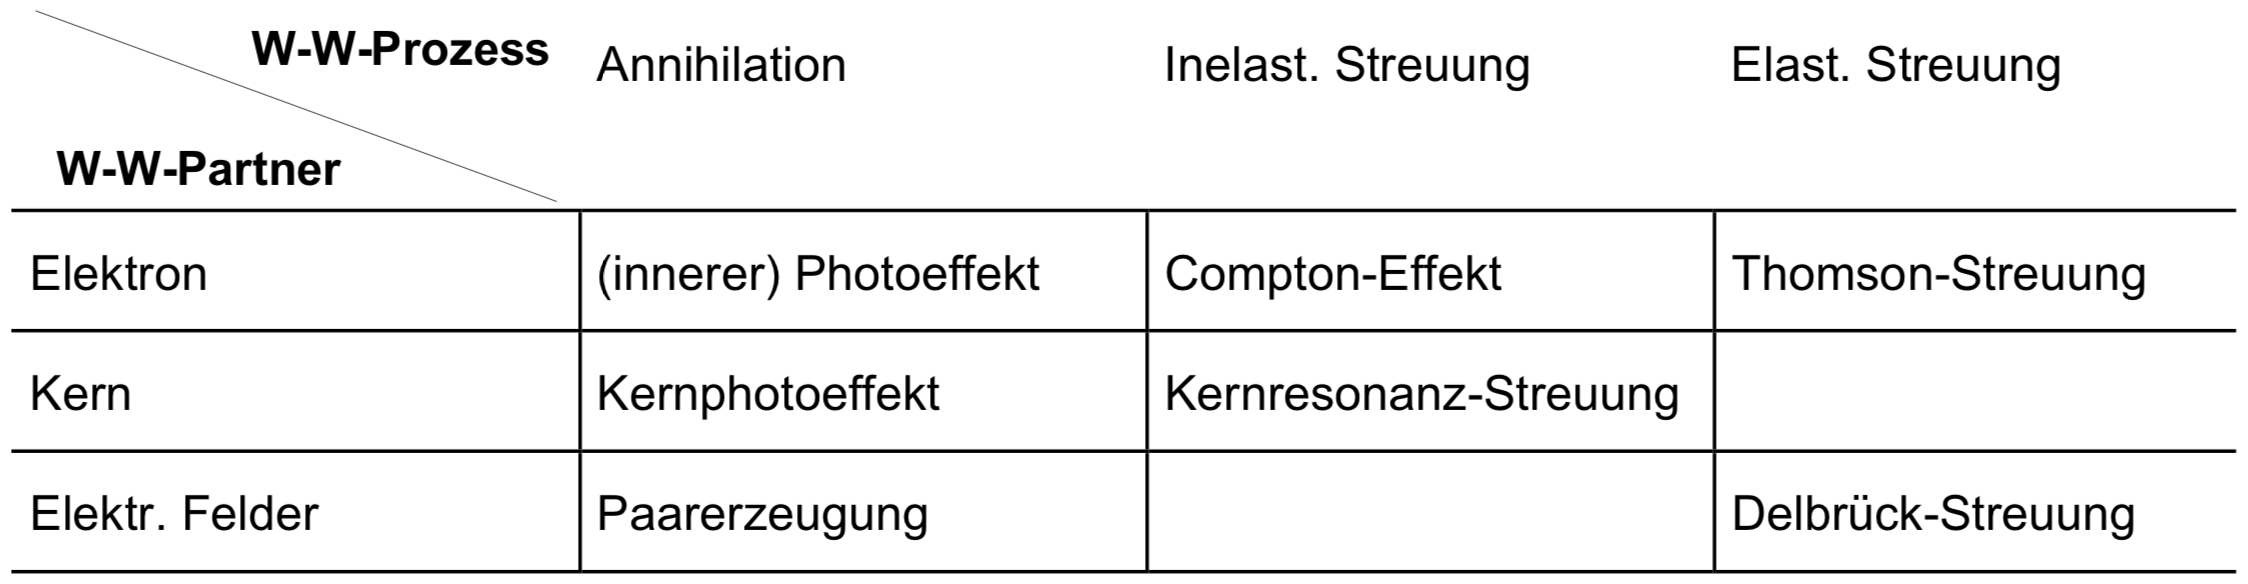
\includegraphics[width=\textwidth]{data/wechselwirkung.png}
  \caption{Verschidene Wechselwirkungen zwischen $\gamma$-Strahlung und Materie \cite{Versuchsanleitung}.}
  \label{fig:wechselwirkung}
\end{figure}

Dabei treten der Photoeffekt, der Compton-Effekt und die Paarbildung am häufigsten auf.
Beim Photoeffekt wird ein $\gamma$-Quant von einem Hüllenelektron des Absorbermaterials
absorbiert und erhält seine Energie. Ist die Energie des Quants dabei höher als die
Bindungsenergie des Elektrons, so kann es aus dem Atom herausgelöst werden. Die
restliche Energie wird in kinetische Energie des Elektrons umgewandelt. Der Photoeffekt
tritt insbesondere bei geringen Energien der $\gamma$-Quanten auf.

Beim Compton-Effekt wird ein $\gamma$-Quant an einem freien Elektron gestreut.
Dabei trifft ein $\gamma$-Quant der Energie $h \nu$ auf ein ruhendes Elektron.
Nach dem Stoßvorgang, besitzt das $\gamma$-Quant nur noch eine Energie von $h \nu' < h \nu$.
Die fehlende Energie liegt nun in Form eines Impulses des Elektrons vor. Die Quanten
werden dabei in unterschiedliche Richtungen gestreut, was zu einer Intensitätsabnahme
des Strahls führt. Der Wirkungsquerschnitt für die Compton-Streuung ist gegeben
durch
\begin{equation}
  \sigma_{\symup{com}}= 2 \pi r_{\symup{e}}^2 \left(\frac{1+\epsilon}{\epsilon^2}
  \left(\frac{2(1+\epsilon)}{1+2\epsilon}-\frac{1}{\epsilon}\ln(1+2\epsilon)\right)
  +\frac{1}{2\epsilon}\ln(1+2\epsilon)-\frac{1+3\epsilon}{(1+2\epsilon)^2}\right) \,.
  \label{eqn:sigma_compton}
\end{equation}
Dabei ist $\epsilon$ das Verhältnis zwischen der Energie des $\gamma$-Quants und
der Ruheenergie des Elektrons und $r_{\symup{e}} = 2,82 \cdot 10^(-15)$m%\frac{e_0^2}{4 \pi \epsilon_0 \m_0 c^2}$
der klassische Elektronenradius. Der Absorptionskoeffizient, für die Absorption, die
durch den Compton-Effekt hervorgerufen wird, ergibt sich zu
\begin{equation}
  \mu_{\symup{com}}=n \sigma_{\symup{com}}(\epsilon) \,.
  \label{eqn:mucompton}
\end{equation}
Der Compton-Effekt ist bei mittleren Energien der $\gamma$-Quanten dominant.

Bei hohen Quantenenergien tritt insbesondere die Paarbildung auf. Dabei können aus
einem $\gamma$-Quant ein Elektron und ein Positron gebildet werden, wobei das
$\gamma$-Quant verschwindet. Die Quantenenergie muss dafür mindestens das doppelte
der Ruheenergie eines Elektrons betragen.

In Abbildung \ref{fig:gamma} ist der Absorptionskoeffizient von Germanium in
Abhängigkeit von der Energie der Strahlung dargestellt.


\begin{figure}
  \centering
  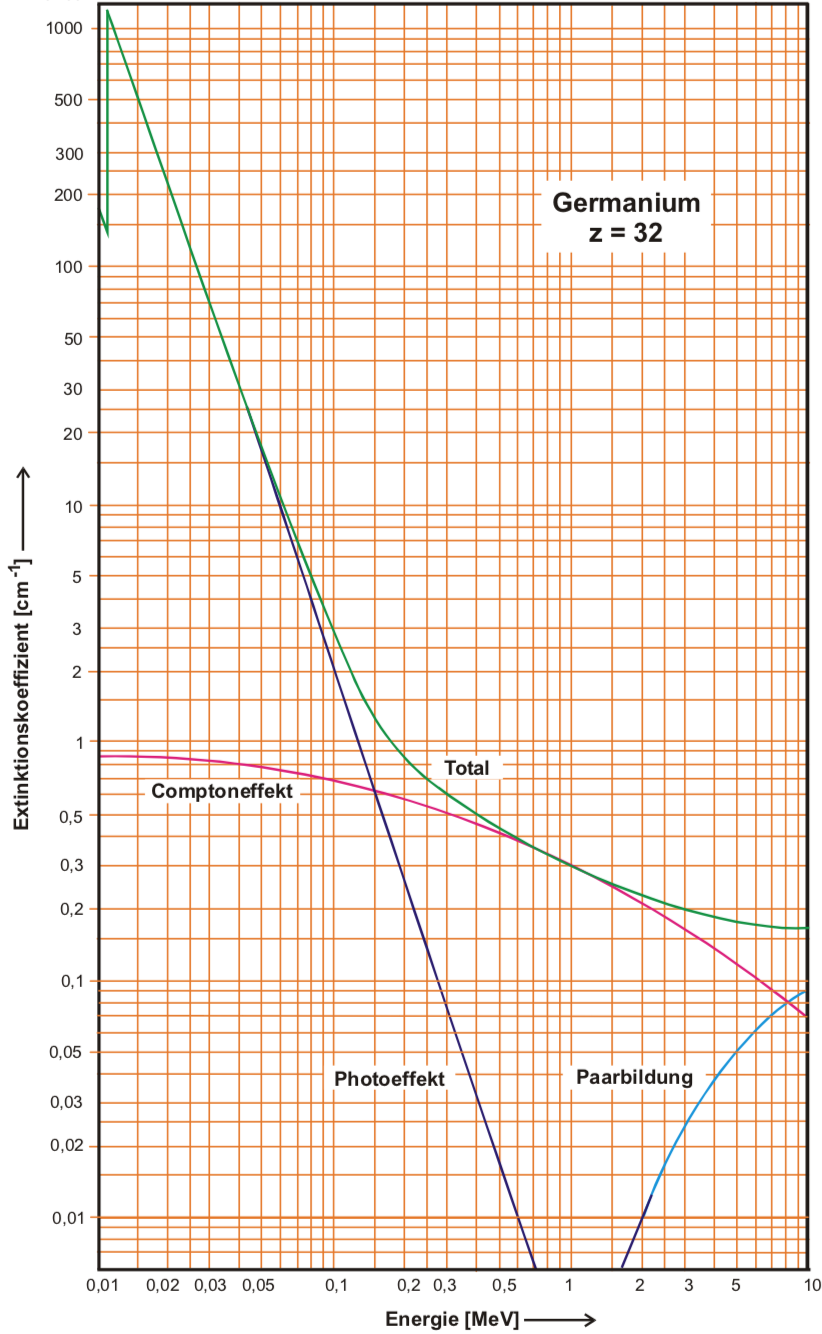
\includegraphics[width=9cm]{data/germanium.png}
  \caption{Absorptionskoeffizient von Germanium in Abhängikeit von der Energie
  der Strahlung \cite{Versuchsanleitung}.}
  \label{fig:gamma}
\end{figure}


\subsection{Theoretische Grundlagen der Beta-Strahlung} % \beta-Strahlung}
\label{subsec:beta}

$\beta$-Strahlung ensteht, wenn im Kern eines Atoms ein Neutron zu einem Proton, einem
Elektron und einem Antineutrino oder aber ein Proton zu einem Neutron, einem Positron
und einem Neutrino zerfällt. Dabei ist der zuerst genannte Prozess energetisch günstiger
und damit wahrscheinlicher. Daher wird im Folgenden auch von diesem Prozess ausgegangen.
Die freiwerdende Energie verteilt sich statistisch auf das Elektron und das Antineutrino.
Daher besitzt $\beta$-Strahlung
ein kontinuierliches Spektrum. Die maximale Energie $E_{\symup{max}}$, die ein
Elektron dabei erhalten kann entspricht der insgesamt beim Zerfall freiwerdenden Energie.

Trifft $\beta$-Strahlung auf Materie, so kann es zu verschiedenen Prozessen kommen.
Einer dieser Prozesse ist die elastische Streuung am Atomkern. Dabei werden die
Elektonen der $\beta$-Strahlung im Coulomb-Feld der Atomkerne gestreut, sodass der
Strahl aufgefächert wird und an Intensität verliert. Zudem werden durch die Streuungen
die Wege der Elektronen durch den Absorber deutlich länger.

Auch inelastische Streuungen an den Atomkernen des Absorbermaterials sind möglich.
Durch die Beschleunigungen der Elektronen im Coulomb-Feld der Atome des Absorbers
wird Energie in Form von elektromagnetischer Strahlung abgegeben. Diese wird auch
Bremsstrahlung genannt.

Der letzte mögliche Prozess ist die inelastische Streuung an den Elektronen des
Absorbers. Dabei werden einzelne Atome des Absorbers ionisiert und angeregt.

Für natürliche $\beta$-Strahlung und eine geringe Schichtdicke $D$ gilt der
Zusammenhang \eqref{eqn:absorptionsgesetz}. Eine typische
Absorptionskurve für $\beta$-Strahlung ist in Abbildung \ref{fig:absorptionskurve}
dargestellt.

\begin{figure}
  \centering
  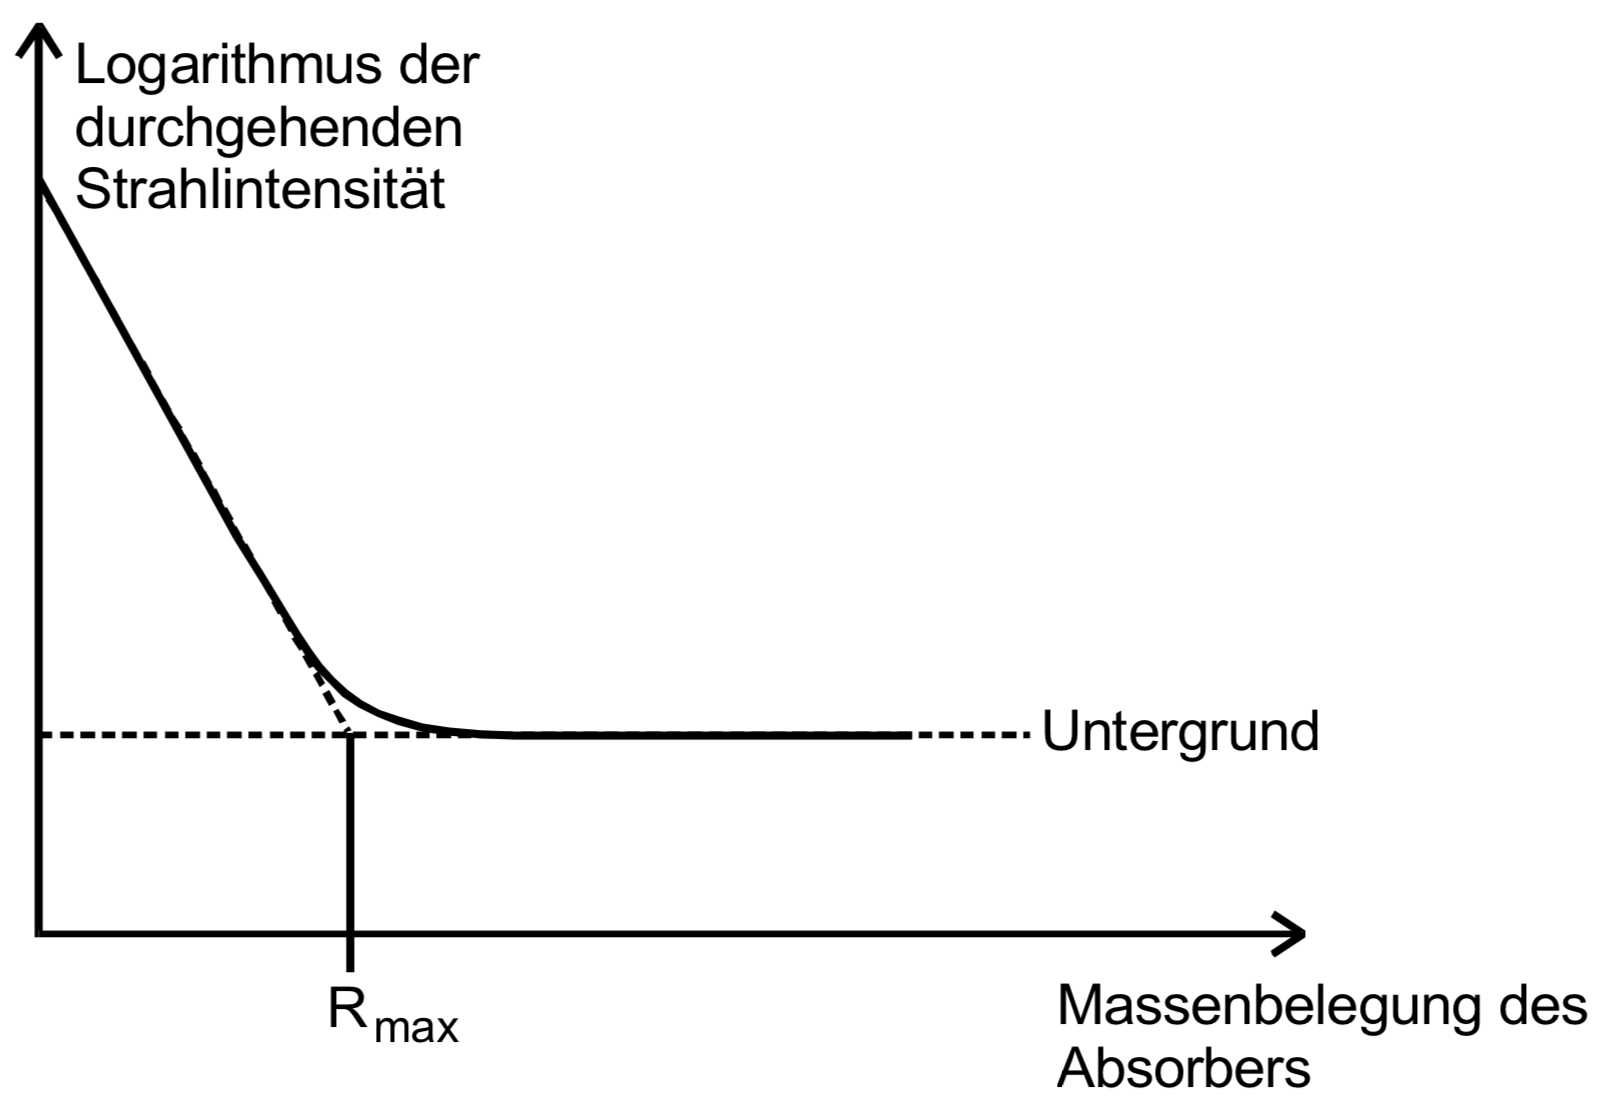
\includegraphics[height=4cm]{data/absorptionskurve.png}
  \caption{Typische Absorptionskurve für natürliche $\beta$-Strahlung \cite{Versuchsanleitung}.
  Die Skalen sind logarithmisch gewählt.}
  \label{fig:absorptionskurve}
\end{figure}

Die Massenbelegung $R$ des Absorbers ist dabei definiert als
\begin{equation}
  R=\rho D \,,
\end{equation}
wobei $D$ die Dicke und $\rho$ die Dichte des Absorbermaterials sind. Die in der Abbildung
als Untergrund gekennzeichnete Strahlung stammt nicht von der $\beta$-Strahlung an sich,
sondern besteht aus Bremsstrahlung und Hintergrundstrahlung.

Ist die maximale Reichweite $R_{\symup{max}}$ bekannt, so lässt sich aus ihr mithilfe
der empirischen Formel
\begin{equation}
  E_{\symup{max}}=1,92 \sqrt{R_{\symup{max}}^2+0,22 R_{\symup{max}}}
  \label{eqn:emax}
\end{equation}
die maximale Energie $E_{\symup{max}}$ des $\beta$-Strahlers in MeV berechnet werden.
